\chapter{State of the art}
\label{chap:soa}

This chapter will begin by analyzing SQL dialects present in some
industry products for event processing --- Coral8 \cite{coral8:www},
StreamBase \cite{streambase:www} and Esper \cite{esper:www}. The
document proceeds with StreamBase EventFlow --- a method for creating
queries visually through a boxes and arrows interface. Despite not
involving programming languages, it's important to study these
alternatives because, after all, they're trying to address the same
problem. Next we describe Oracle Rules Manager with its rule-based
paradigm for complex event processing. We will conclude this chapter
analyzing MonitorScript, a procedural language developed by Progress
Apama with the intention of overcoming the limitations imposed by
SQL-like languages.

\section{SQL-based languages}
\label{sec:sql}

The most popular way of writing queries for ESP applications is
through SQL dialects. As explained in the introduction, this comes as
a result of all the effort the database community has invested into
ESP. Besides creating the first event processing systems, this
commitment produced few languages, most notably CQL -- the Continuous
Query Language \cite{cql} used by Stanford's STREAM
\cite{stream}. Other research projects using SQL dialects include
Gigascope \cite{gigascope} from AT\&T Labs and TelegraphCQ
\cite{telegraphcq} developed at Berkeley. Currently there is no
standard for a query language designed specifically for these
applications, which means each vendor has their own. Fortunately,
they're all very similar. The simplest things can be done in a very
similar way to SQL:

\lstset{
  language=CCL,
  columns=fullflexible,
  basicstyle=\tt,
  keywordstyle=[1]\bf,
  keywordstyle=[2]\it,
}

\begin{lstlisting}
  insert into PriceACME
  select *
  from   StockTrades
  where  symbol = 'ACME'
\end{lstlisting}

This query looks for tuples where the field \verb=symbol= equals
``ACME'' arriving at the stream \verb=StockTrades= and adds them to
the \verb=PriceACME= stream. It's just a simple filter that separates
ACME events from the others.

We've been talking a lot about streams without defining
them. Conceptually, streams are channels where events flow from one
endpoint to another. We may tap into these channels and gather data,
or derive new information -- which is essentially the point of writing
queries. Typical event processing applications are not transient by
nature -- quite on the contrary: they can go on for days, months,
years even, always receiving events and performing calculations. As
such, queries in this domain are said to be \emph{continuous} -- i.e.,
they are always active while the application is running. This is very
different from what happens in a typical DBMS, where queries are
short-lived and execute over discrete units of time.

Unlike database tables, streams don't store events: as soon as an
event is processed, it is discarded. However, we may use
\emph{windows} to buffer events. Windows are similar to tables, but
they come with a few extras that turn out to be useful in the domain
of event processing. In particular, windows provide constructs to
manage recent data and perform calculations over it. This way, it
becomes very easy, for example, to calculate the most expensive order
among the last million, or the average of ACME's stock prices over the
last 3 hours, as the following listing shows:

\begin{lstlisting}
  insert into AvgPriceACME
  select avg(price)
  from   StockTrades keep 3 hours -- Window creation!
  where  symbol = 'ACME'
\end{lstlisting}

More advanced windows allow the developer to retain, for example, the
10 largest updates based on their price, the 10 last updates per
company or simply to keep everything.

The window defined in the previous example is a \emph{sliding}
window. Sliding, in this context, refers to how and when the elements
in the window expire. In these kinds of windows, tuples are removed
from the window as they become too old or new tuples arrive. An
alternative is \emph{jumping} windows, where tuples are appended to
the window and then, when the oldest element was supposed to be
removed, all of them expire at the same time, the window becomes empty
and the cycle begins all over again. This way, it's possible to find
out the largest price attained by each company over the last hour, the
hour before and so on:

\begin{lstlisting}
  insert into MaxPrices
  select symbol, max(price)
  from StockTrades keep every 1 hour -- Note the keyword every
  group by symbol
  output every 1 hour;
\end{lstlisting}

All the examples in this section were written in Coral8 Continuous
Computation Language (CCL) \cite{coral8-ccl:www}. Nonetheless, all the
other systems in this section provide similar features albeit with
different syntax. In fact, there have been talks about creating a
standard language lately, an idea that was met with some skepticism
\cite{sql-impendance-mismatch:post}.

With the undeniable increasing relevance of ESP and the predominance
of SQL-based languages in currently-available products, it is
important to analyze their limitations. After all, it doesn't make
sense to build yet another programming language if the existing ones
are good enough. This will be the topic of the next chapter.

\section{Building queries visually with StreamBase's EventFlow}
\label{sec:eventflow}

StreamBase employs an alternative, more user-friendly, way of building
queries. Instead of writing code, the user can design queries
visually, by arranging boxes in a canvas and connecting them with
arrows. Boxes represent operators that receive data coming from other
operators or directly from the input streams, process the data and
send the results to be handled by other operators, or to the world as
the output of the whole operation. An example is shown in figure
\ref{fig:eventflow-sample}.

\begin{figure}[htbp]
  \centering
  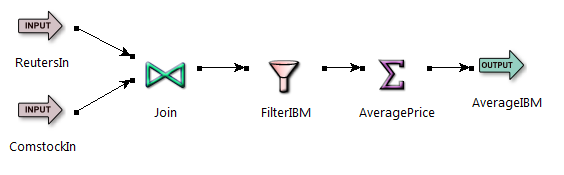
\includegraphics[width=\textwidth]{eventflow.png}
  \caption{This diagram represents a simple query where two streams
    are joined, non IBM tuples are filtered-out, and then the average
    of IBM stock prices over the last 5 minutes is sent to the
    output.}
  \label{fig:eventflow-sample}
\end{figure}

Some of the most important operators are:

\begin{description}
\item [Aggregate] Computes aggregate operations over windows of
  tuples. Supports the option to partition tuples into sets and then
  apply the aggregation over each individual set, much like a SQL
  GROUP BY statement;
\item [Filter] Discards some tuples from the input stream based on a
  predicate. Performs the same function as a SQL WHERE statement;
\item [Gather] Receives tuples from two or more streams and
  concatenates those with the same key. The resulting tuple values may
  be direct copies from the original tuples or the result of applying
  some expression to these;
\item [Join] Similar to SQL joins, this operator pairs tuples coming
  from two streams that match a given condition and outputs a new
  tuple whose fields may be specified by the user. In general, joining
  two infinite streams may require keeping all tuples from both
  streams in memory. To avoid problems later on, the user must specify
  timing constraints regarding matching tuples saying, for example,
  that they must arrive within 60 seconds of each other;
\item [Map] Similar to the first part of a SELECT statement, this
  operator transforms a tuple --- possibly discarding or adding new
  fields along the way ---, and sends it downstream;
\item [Pattern] Instructs the engine to look for specific patterns of
  events;
\item [Union] Acts as a multiplexer, connecting many input streams to
  a single output stream, to where all tuples are sent. Similar to the
  SQL UNION statement.
\end{description}

It's clear that most of these operators have SQL counterparts. There
are a few things that can be done in EventFlow but not in StreamSQL
(see the online documentation at \cite{eventflow2streamsql}), but
they're just small details, nothing that changes the developer's way
of thinking. It's then mostly a matter of taste --- not power ---, to
choose between StreamSQL and EventFlow.

\section{Oracle rules}
\label{sec:orm}

Oracle Rules Manager (ORM) \cite{orm:www} embraces a completely
different paradigm. Instead of writing queries, the user creates rules
that are made of three parts. The first, the event type, instructs the
system to trigger the rule only when an event of that type occurs. The
second, the condition, is a predicate that is compared against the
event. If they match, the third part, the action --- a PL/SQL
procedure ---, is executed.

Conceptually, a rule has the following format:

\lstset{
  language=Oracle,
  columns=fullflexible,
  basicstyle=\tt,
  keywordstyle=\bf,
}


\begin{lstlisting}
  on   <event>
  if   <condition>
  then <action>
\end{lstlisting}

The following example shows a simple rule:

\begin{lstlisting}
  on   StockTick(symbol, price)
  if   symbol = 'ACME' and price > 100
  then buyStocks(symbol)
\end{lstlisting}

The event shown above represents a stock update received from some
external source. These are the simplest kind of events, also called
\emph{primitive} events. ORM also supports \emph{composite} events
that are defined as combinations of other events. For example, it is
possible to define a composite event that occurs when ACME shares drop
10\% and, less than 5 minutes later, some other company's shares gain
2\%. To be more specific, the following types of combinations are
supported:
\begin{description}
\item [Sequencing] Specifies the order between events, i.e., event A
  must occur before event B;
\item [Negation] Checks for the non-occurrence of some event. Useful
  to raise exceptions when business rules are violated;
\item [Set semantics] Allows combining events with the AND operator to
  specify that all of them must occur for the composite event to occur
  as well;
\item [Any N] Checks for the occurrence of at least N children events;
\item [Collection] Combines a set of primitive events based on some
  common properties. Could be used, for example, to detect all
  costumers who withdrew more than \$1000 from their bank accounts
  during the past 24h.
\end{description}

ORM comes with a GUI utility to simplify the rules creation
process. This is necessary because creating a rule the hard way is a
daunting task that involves writing SQL queries containing XML blocks
containing SQL snippets inside. Still, there are situations when one
needs to avoid these utilities and work with real code, situations
where a simpler configuration process would be desirable.

The biggest disadvantage of rule-based languages comes from the
paradigm itself. While they may be effective for detecting complex
patterns of events, they are not so good when it comes to actually
processing the data. Built-in combinators provide some aggregation
functions, but these will seem basic for companies in need to
implement proprietary analysis algorithms. Also, PL/SQL is arguably
not a language suited for event-based complex application development.

One other issue that hinders these systems is the difficulty to reason
about their runtime behavior. As the number and complexity of rules
increases, an event may trigger more than one rule and these rules may
themselves trigger other rules, resulting in a cascading process that
may never end. This behavior makes the applications more difficult to
understand, to the point where even adding or removing a simple rule
may have unpredictable effects. These kinds of non-linear interactions
are discouraged by Software Engineering best-practices and thus, the
decision to use rule-based systems for building large applications
must be carefully pondered. To be fair, Oracle Rules Manager provides
constructs to deal with simultaneous triggering rules, but the problem
doesn't go away.

\section{Apama's MonitorScript}

When ESP solutions left the academia to meet the real world, many
users argued that SQL-based languages were ill-suited for many
information processing tasks. MonitorScript (MS) is Apama's response
to these complains.

Deriving from the procedural family of programming languages, MS
programs look a lot like Java programs. However, the most important
and unique feature it includes is the actor model based on having many
little \emph{processes} that execute in parallel and communicate with
each other through messages. In MS, these entities are called
\emph{monitors}. A monitor is an event processing agent that basically
sets up an arbitrary number of \emph{listeners} that await for the
occurrence of events. When one matching event arrives, monitors
process it. Monitors can also send events to each other, through the
\emph{route} statement.

Last but not least, monitors can have state. This means that instead
of writing a SQL query to capture the state of the system, MS updates
the state incrementally as the computation moves forward. The downside
is that, for simple things, SQL queries will definitely be easier to
understand, because a SQL query \emph{is} its intention while, in a
procedural program, the big picture is not always that clear.

To get a feeling for the language, here is a small MonitorScript
snippet:

\lstset{
  language=MonitorScript,
  columns=fullflexible,
  basicstyle=\tt,
  keywordstyle=[1]\bf,
  keywordstyle=[2]\it,
}


\begin{lstlisting}
monitor ProcessMarket {
    // Keep the last price per company
    dictionary <string, int> lastPerCompany;

    action onload {
        Tick tick;
        on all Tick(): tick {
           processTick(tick);
        }

        on all PriceRequest(): ev {
            processPriceRequest(ev);
        }
    }

    action processTick(Tick tick) {
        lastPerCompany[tick.sym] := tick.price;
        route TickAck(tick.sym);
    }

    action processPriceRequest(PriceRequest ev) {
        if (lastPerCompany.hasKey(ev.sym)) then {
            route PriceReply(ev.sym, lastPerCompany[ev.sym]);
        }
    }
}
\end{lstlisting}

This listing declares one monitor (\verb=ProcessMarket=), that waits
for \verb=Tick= and \tt Last- PriceRequest \rm events. When it receives a
new \verb=Tick= update, it keeps the price reported in a dictionary,
indexed by the company's symbol and replies with a \verb=TickAck=
message. When it receives a \verb=PriceRequest=, it fetches the last
price from the dictionary and sends a \verb=PriceReply= message.

Note the need to create request, reply and acknowledgment messages
when what one really wants to do is to perform a method invocation
between different monitors. Indeed, the runtime system could provide
some kind of remote procedure call mechanism and handle the low-level
details by itself.

MS and SQL are at opposite ends of the programming language
spectrum. While it simplifies a lot of tasks that don't naturally fit
into SQL, MS also looses all the querying capabilities that made SQL
and its derivatives popular for data processing.
